% Overleaf-ready standalone section for the WormShield paper.
% Upload this file together with the PNG assets in ./figures/.
% Required packages: graphicx, booktabs

\documentclass[10pt]{article}
\usepackage[margin=1in]{geometry}
\usepackage{graphicx}
\usepackage{booktabs}
\usepackage[T1]{fontenc}
\usepackage[utf8]{inputenc}

\title{WormShield Detection Pipeline}
\author{}
\date{}

\begin{document}
\maketitle

\section{WormShield}
\label{sec:wormshield}

WormShield is a lightweight decision-time detector for semantic worm propagation in multi-agent AI systems. Its goal is narrower than generic harmful-content moderation: given a local relay step, WormShield predicts whether the current node is still preserving a payload in a form that can continue spreading downstream. For the main detector, we collapse the AgentArena labels into a binary task with \texttt{propagating}=1 and \texttt{clean}/\texttt{exposed}=0. This choice keeps the positive class aligned with active onward spread rather than with mere exposure to suspicious content.

\subsection{Feature Construction}

The final shared pipeline combines three branches: a semantic branch, a lexical overlap branch, and a lightweight response-length branch. Figure~\ref{fig:wormshield-pipeline} summarizes the design. On AgentArena, the semantic text view is built by concatenating the incoming message, the local model output, and the forwarded message, which lets the embedding branch observe paraphrastic retention across the relay step. On Here-Comes-the-AI-Worm, the same pipeline family is used, but the semantic text view is instantiated from the reply field provided by that dataset. In both cases, the semantic branch encodes the text view with \texttt{sentence-transformers/all-MiniLM-L6-v2}.

The lexical branch computes seven portable similarity features: Jaccard, BLEU, ROUGE-1, ROUGE-2, ROUGE-L, METEOR, and Jaro-Winkler. These metrics preserve compatibility with DonkeyRail-style text-similarity defenses while expanding beyond a single scalar score. The length branch adds four inexpensive response-shape features: character length, token length, unique-token count, and average token length. We then concatenate the selected branch outputs into one numeric feature vector and train a portable XGBoost classifier.

\begin{figure}[t]
    \centering
    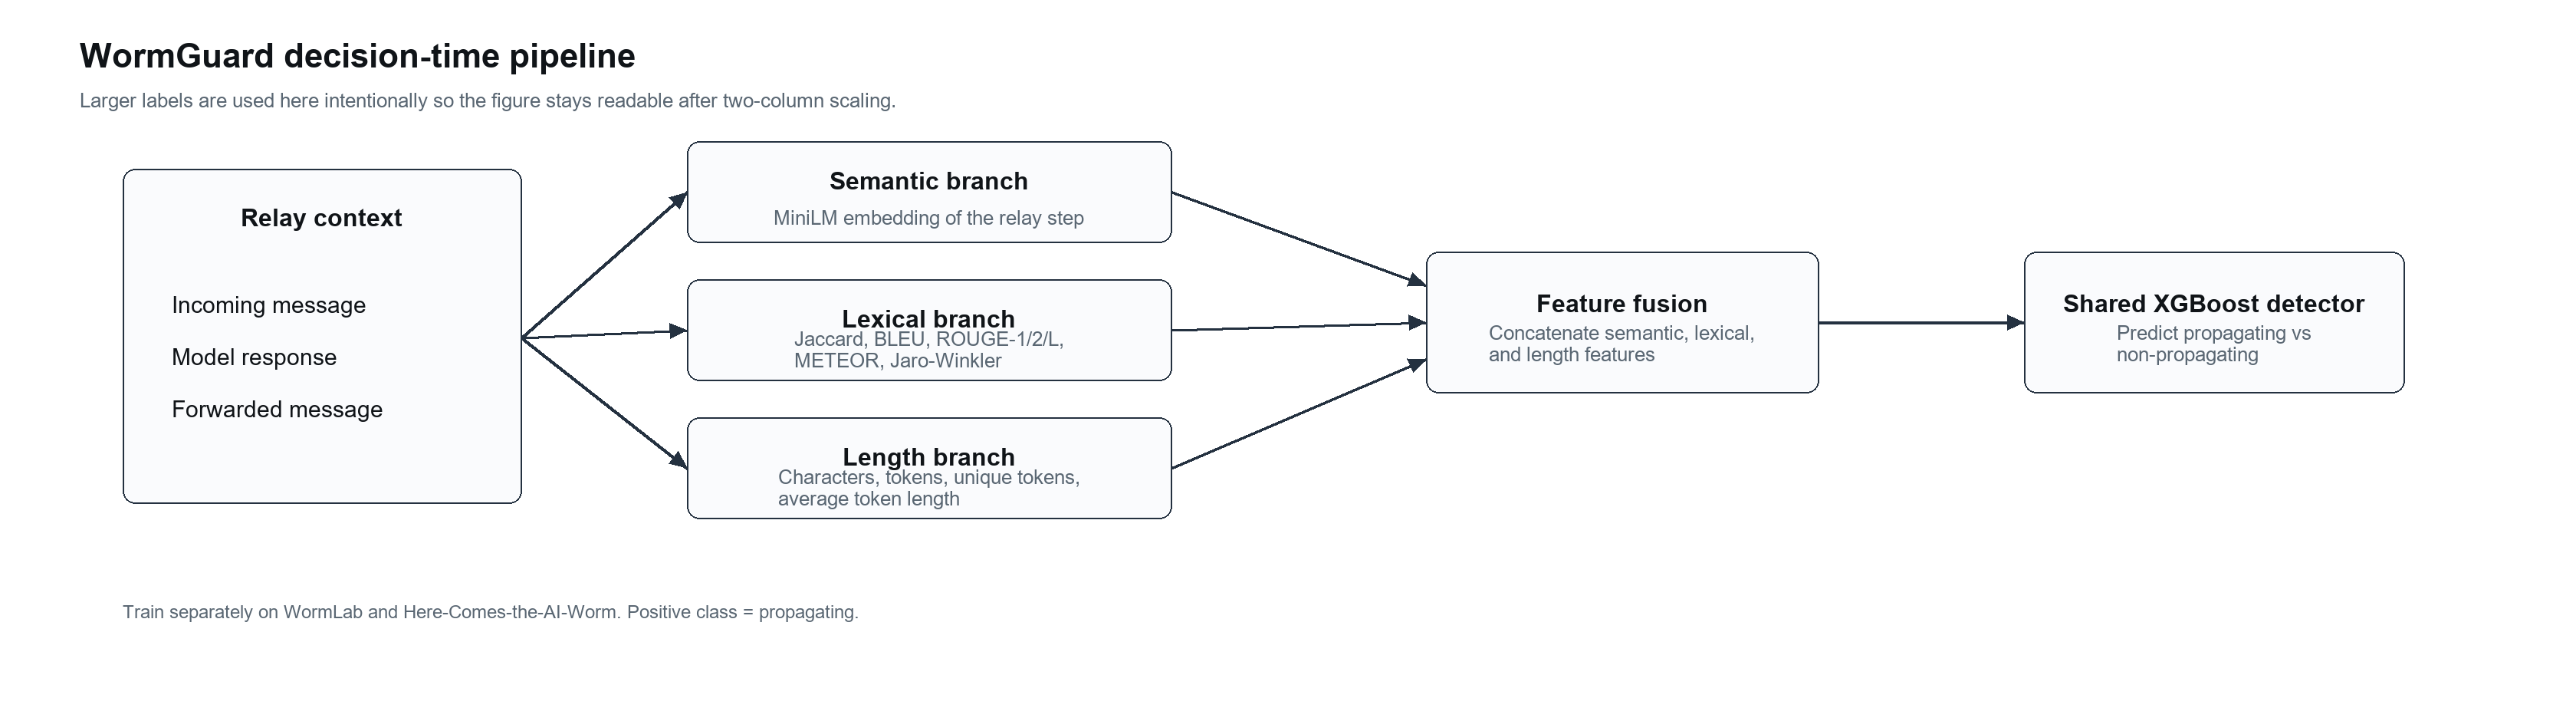
\includegraphics[width=\linewidth]{figures/wormshield-pipeline-figure.png}
    \caption{Paraphrase-aware WormShield pipeline. The detector fuses a semantic embedding branch, a lexical similarity branch, and a lightweight length branch, and predicts whether the current relay step is still propagation-capable.}
    \label{fig:wormshield-pipeline}
\end{figure}

\subsection{Training Protocol}

We train the same detector family separately on AgentArena and Here-Comes-the-AI-Worm so that the comparison isolates feature design rather than mixing training corpora. AgentArena uses grouped-by-run train/validation/test splits, while Here-Comes-the-AI-Worm uses grouped-by-person validation splits with the official test set kept fixed. To reduce seed sensitivity, every shared-pipeline result is repeated over five seeds \{7, 19, 31, 43, 59\}, and the reported values are mean $\pm$ standard deviation. Rather than keeping only a single ``best DonkeyRail'' summary row, we compare against the full lightweight classifier family emphasized by Here-Comes-the-AI-Worm: Logistic Regression, Naive Bayes, and Decision Stump. On AgentArena, these rows come from the official DonkeyRail family adapted to the same split; on Here-Comes-the-AI-Worm, the matching fixed-threshold rows are taken from the released test tables.

We considered three lexical variants and three paraphrase-aware variants. The lexical family tests how far a shared similarity-only design can go when trained identically on both datasets. The paraphrase-aware family adds the MiniLM semantic branch to capture relay-preserving rewrites and paraphrases, which are especially common in AgentArena. The selected main variant is \texttt{semantic\_plus\_similarity7\_plus\_lengths}, because it gives the strongest overall cross-dataset validation behavior while remaining small and easy to ablate.

\subsection{Main Results}

Table~\ref{tab:wormshield-agentarena-main} shows the AgentArena comparison. All three official DonkeyRail-family baselines remain well below the paraphrase-aware WormShield variant on accuracy, precision, F1, ROC-AUC, and false-positive rate. Among the lightweight baselines, Decision Stump gives the strongest recall and F1, while Logistic Regression and Naive Bayes keep false positives lower but remain far weaker overall. This is the main result that matters for the AgentArena setting, because the dataset contains rewritten and paraphrased propagation traces that are not well captured by lexical overlap alone.

\begin{table}[t]
\centering
\small
\setlength{\tabcolsep}{4pt}
\caption{AgentArena main comparison. Official DonkeyRail-family rows are evaluated on the same AgentArena split, and shared-pipeline rows report five-seed mean $\pm$ std. Best values are bolded; lower is better for FPR.}
\label{tab:wormshield-agentarena-main}
\begin{tabular}{lcccccc}
\toprule
Model & Accuracy & Precision & Recall & F1 & ROC-AUC & FPR \\
\midrule
Logistic Regression & 0.7179 & 0.5351 & 0.4296 & 0.4766 & 0.8045 & 0.1592 \\
Naive Bayes & 0.7200 & 0.5354 & 0.4789 & 0.5056 & 0.8045 & 0.1786 \\
Decision Stump & 0.7326 & 0.5339 & \textbf{0.8310} & 0.6501 & 0.7608 & 0.3436 \\
Shared lexical XGB & 0.6967 $\pm$ 0.0301 & 0.4916 $\pm$ 0.0451 & 0.6096 $\pm$ 0.0246 & 0.5429 $\pm$ 0.0273 & 0.7563 $\pm$ 0.0184 & 0.2669 $\pm$ 0.0442 \\
Paraphrase-aware WormShield & \textbf{0.9027 $\pm$ 0.0097} & \textbf{0.8597 $\pm$ 0.0227} & 0.8013 $\pm$ 0.0281 & \textbf{0.8290 $\pm$ 0.0161} & \textbf{0.9579 $\pm$ 0.0060} & \textbf{0.0547 $\pm$ 0.0099} \\
\bottomrule
\end{tabular}
\end{table}

Table~\ref{tab:wormshield-aiworm-main} shows the corresponding comparison on Here-Comes-the-AI-Worm. Here we expand the baseline set to the explicit classifier rows reported in the released DonkeyRail test tables: Logistic Regression with ROUGE-L plus METEOR, Naive Bayes with METEOR, and Decision Stump with BLEU plus METEOR. On this benchmark, the shared XGBoost family outperforms the published fixed-threshold baselines on accuracy, precision, F1, and false-positive rate, while the published Logistic Regression and Naive Bayes rows retain slightly higher recall and the strongest ROC-AUC. The paraphrase-aware variant remains close to the lexical shared model and slightly improves ROC-AUC over it. This pattern is consistent with the fact that Here-Comes-the-AI-Worm is less paraphrase-heavy than AgentArena.

\begin{table}[t]
\centering
\small
\setlength{\tabcolsep}{4pt}
\caption{Here-Comes-the-AI-Worm main comparison. Published DonkeyRail-family rows are taken from the released fixed-threshold test tables, and shared-pipeline rows report five-seed mean $\pm$ std. Best values are bolded; lower is better for FPR.}
\label{tab:wormshield-aiworm-main}
\begin{tabular}{lcccccc}
\toprule
Model & Accuracy & Precision & Recall & F1 & ROC-AUC & FPR \\
\midrule
Logistic Regression & 0.9742 & 0.9523 & \textbf{0.9938} & 0.9726 & \textbf{0.9953} & 0.0454 \\
Naive Bayes & 0.9734 & 0.9509 & \textbf{0.9938} & 0.9719 & 0.9950 & 0.0450 \\
Decision Stump & \textbf{0.9806} & 0.9653 & \textbf{0.9938} & 0.9793 & 0.9816 & 0.5085 \\
Shared lexical XGB & 0.9804 $\pm$ 0.0015 & \textbf{0.9729 $\pm$ 0.0005} & 0.9916 $\pm$ 0.0031 & \textbf{0.9822 $\pm$ 0.0014} & 0.9861 $\pm$ 0.0002 & \textbf{0.0329 $\pm$ 0.0007} \\
Paraphrase-aware WormShield & 0.9800 $\pm$ 0.0016 & 0.9725 $\pm$ 0.0003 & 0.9913 $\pm$ 0.0027 & 0.9818 $\pm$ 0.0014 & 0.9863 $\pm$ 0.0002 & 0.0334 $\pm$ 0.0003 \\
\bottomrule
\end{tabular}
\end{table}

For completeness, the Here-Comes-the-AI-Worm paper also reports a threshold-tuned Virtual Donkey headline operating point with TPR $=1.0$ and FPR $=0.015$, plus a separate out-of-distribution Hillary email evaluation. We do not mix that row into Table~\ref{tab:wormshield-aiworm-main} because the paper does not report fixed-threshold precision or F1 for that operating point.

Figure~\ref{fig:wormshield-main-results} gives a visual view of the expanded comparison over F1, ROC-AUC, and FPR across both datasets. The figure makes the main trade-off clear: semantic features matter a great deal on AgentArena, while the Here-Comes-the-AI-Worm benchmark is already close to saturation for the stronger fixed-threshold baselines.

\begin{figure}[t]
    \centering
    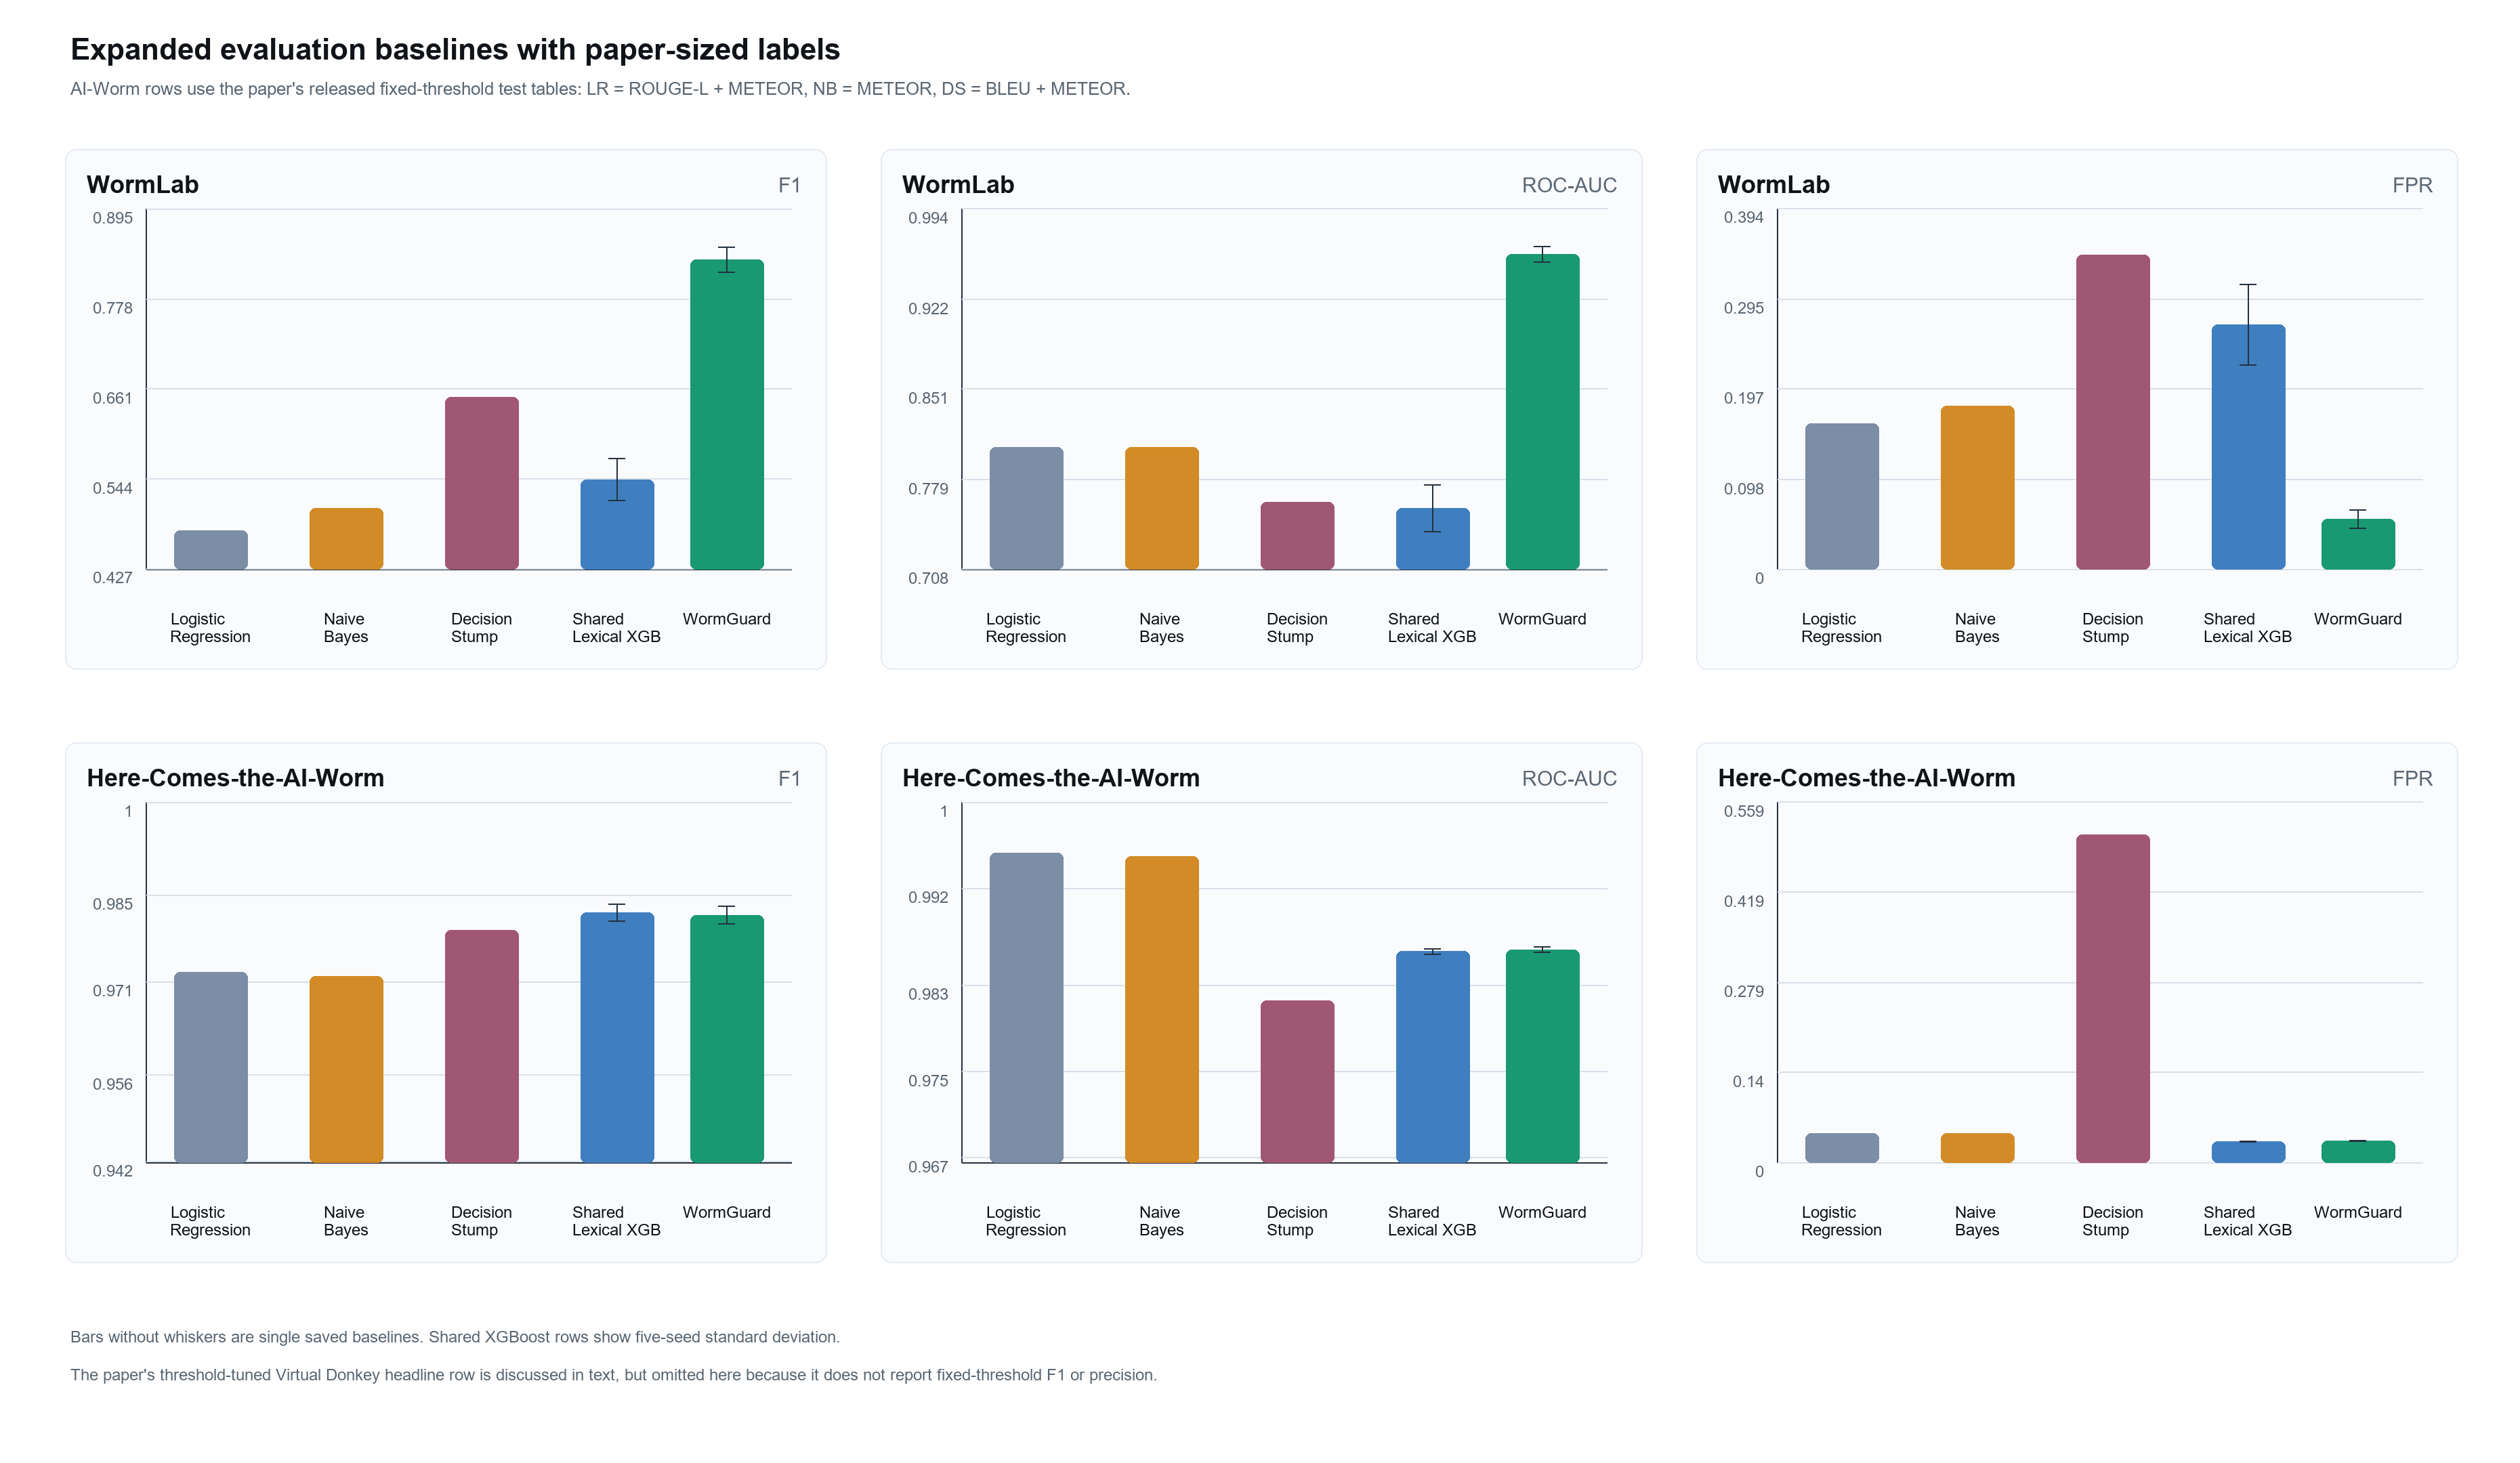
\includegraphics[width=\linewidth]{figures/wormshield-main-results.png}
    \caption{Expanded WormShield comparison on AgentArena and Here-Comes-the-AI-Worm. Each panel includes Logistic Regression, Naive Bayes, Decision Stump, the shared lexical XGBoost model, and paraphrase-aware WormShield. Error bars denote five-seed standard deviation for the shared models.}
    \label{fig:wormshield-main-results}
\end{figure}

\subsection{Ablation on AgentArena}

We use AgentArena for the ablation study because it is the dataset that stresses paraphrastic rewriting most directly. Table~\ref{tab:wormshield-agentarena-ablation} shows that the purely lexical shared family remains well below the semantic family. Adding the embedding branch causes the major jump in F1 and ROC-AUC, which supports the claim that semantic retention rather than surface overlap is the main source of robustness. Within the semantic family, the three best variants are close to each other; adding the lexical and length features slightly improves precision, ROC-AUC, and FPR, while the embedding-only variant keeps the best recall and a nearly tied F1.

\begin{table}[t]
\centering
\small
\setlength{\tabcolsep}{4pt}
\caption{AgentArena ablation study. Best values are bolded; lower is better for FPR. All rows report five-seed mean $\pm$ std.}
\label{tab:wormshield-agentarena-ablation}
\begin{tabular}{lcccccc}
\toprule
Variant & Accuracy & Precision & Recall & F1 & ROC-AUC & FPR \\
\midrule
\texttt{shared\_similarity7} & 0.6890 $\pm$ 0.0260 & 0.4808 $\pm$ 0.0393 & 0.5761 $\pm$ 0.0361 & 0.5220 $\pm$ 0.0170 & 0.7387 $\pm$ 0.0126 & 0.2639 $\pm$ 0.0481 \\
\texttt{shared\_similarity7\_plus\_lengths} & 0.6967 $\pm$ 0.0301 & 0.4916 $\pm$ 0.0451 & 0.6096 $\pm$ 0.0246 & 0.5429 $\pm$ 0.0273 & 0.7563 $\pm$ 0.0184 & 0.2669 $\pm$ 0.0442 \\
\texttt{shared\_similarity7\_plus\_light\_format} & 0.7178 $\pm$ 0.0124 & 0.5203 $\pm$ 0.0229 & 0.6217 $\pm$ 0.0632 & 0.5635 $\pm$ 0.0150 & 0.7707 $\pm$ 0.0141 & 0.2415 $\pm$ 0.0399 \\
\texttt{semantic\_embedding\_only} & 0.9027 $\pm$ 0.0076 & 0.8524 $\pm$ 0.0221 & \textbf{0.8108 $\pm$ 0.0200} & \textbf{0.8307 $\pm$ 0.0121} & 0.9574 $\pm$ 0.0045 & 0.0587 $\pm$ 0.0094 \\
\texttt{semantic\_plus\_similarity7} & \textbf{0.9028 $\pm$ 0.0071} & 0.8537 $\pm$ 0.0270 & 0.8095 $\pm$ 0.0187 & 0.8305 $\pm$ 0.0116 & 0.9577 $\pm$ 0.0057 & 0.0580 $\pm$ 0.0118 \\
\texttt{semantic\_plus\_similarity7\_plus\_lengths} & 0.9027 $\pm$ 0.0097 & \textbf{0.8597 $\pm$ 0.0227} & 0.8013 $\pm$ 0.0281 & 0.8290 $\pm$ 0.0161 & \textbf{0.9579 $\pm$ 0.0060} & \textbf{0.0547 $\pm$ 0.0099} \\
\bottomrule
\end{tabular}
\end{table}

\begin{figure}[t]
    \centering
    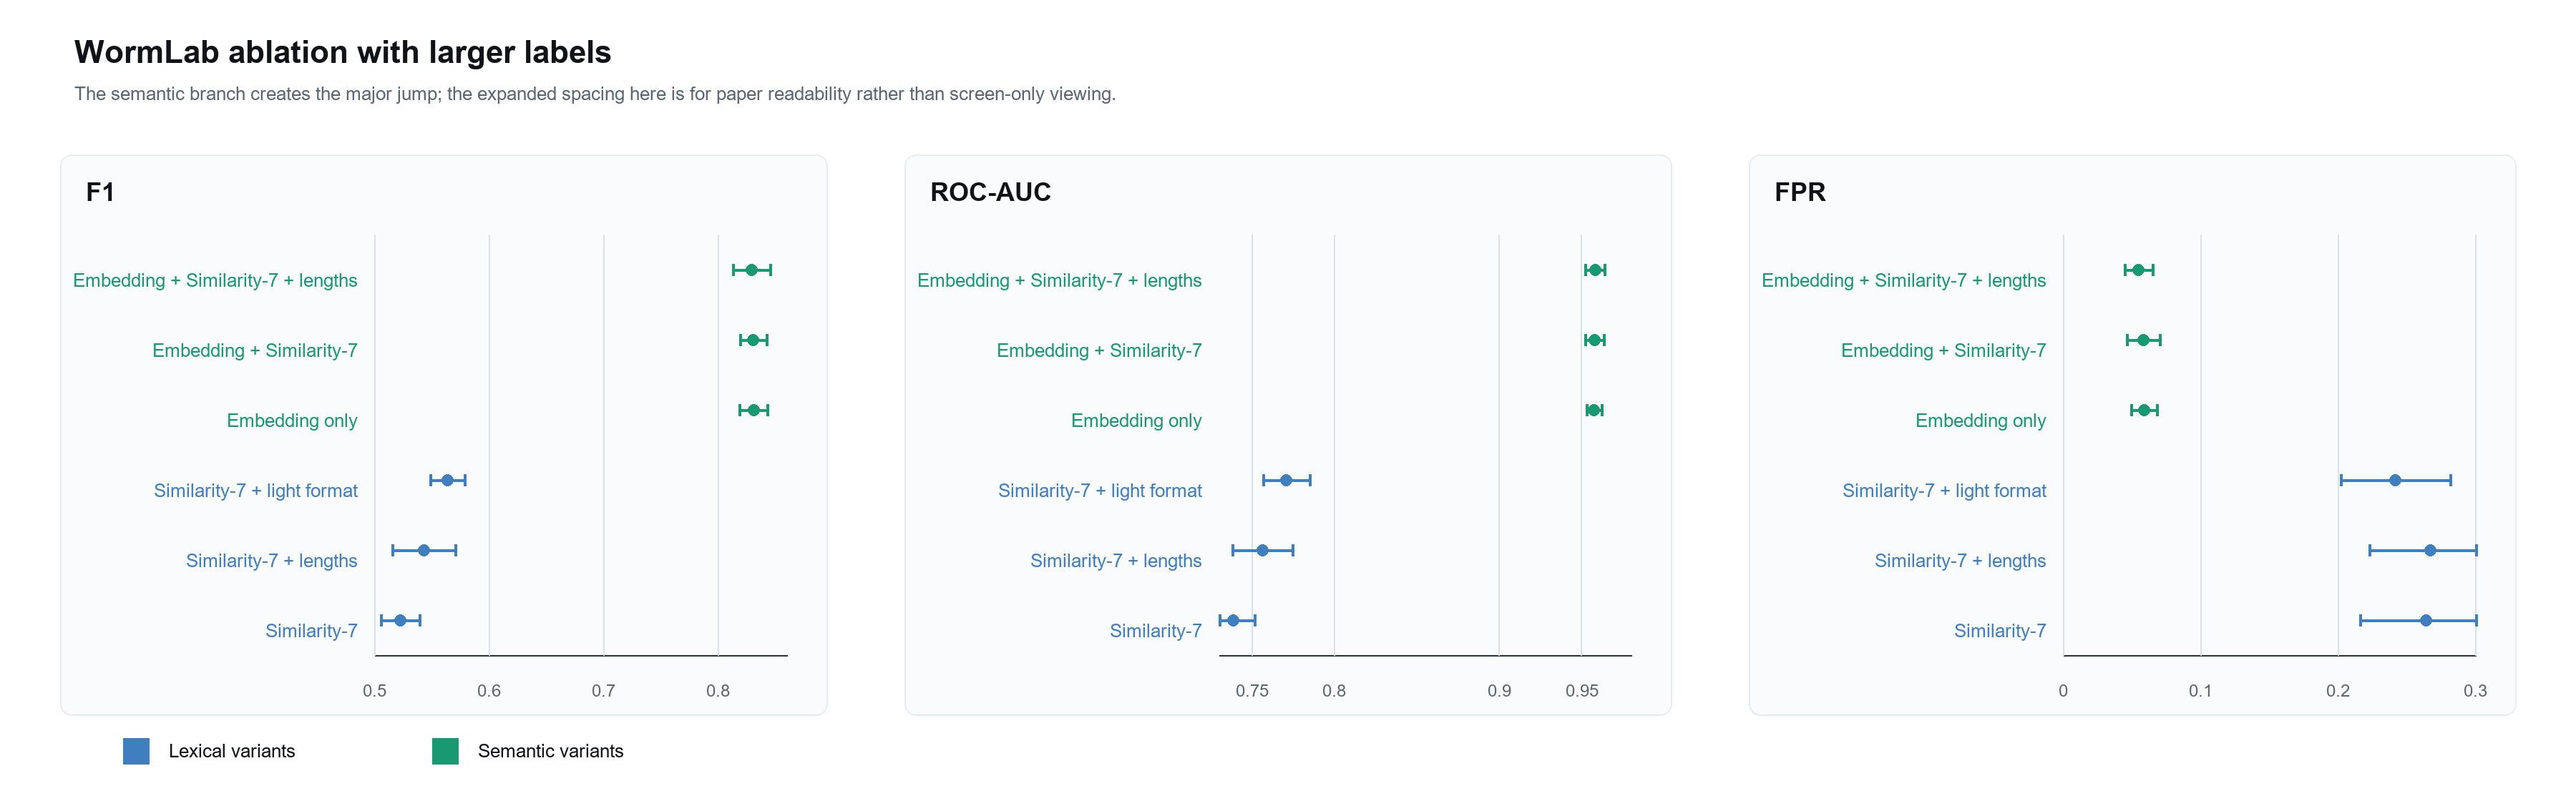
\includegraphics[width=\linewidth]{figures/wormshield-agentarena-ablation.png}
    \caption{AgentArena ablation for the lexical and paraphrase-aware WormShield variants. Panels summarize F1, ROC-AUC, and FPR with five-seed standard-deviation whiskers. The semantic branch produces the dominant gain, while lexical and length features provide smaller refinements within the semantic family.}
    \label{fig:wormshield-agentarena-ablation}
\end{figure}

\subsection{System-Level AgentArena Evaluation}

The preceding experiments evaluate WormShield at the level of individual relay decisions. We additionally evaluate AgentArena at the system level to characterize how semantic worms propagate through different multi-agent communication structures and to determine whether decision-level detection translates into effective containment.

\subsubsection{Effect of Network Topology}

Communication structure has a substantial effect on semantic propagation. Across malicious clean runs, \texttt{mesh\_lite} produces the broadest and deepest cascades, with mean attack reach $0.450$, mean propagating-agent fraction $0.251$, mean maximum depth $6.805$, and mean $2.951$ propagation-capable relay events per run. Ring and \texttt{random\_min\_degree} remain moderately susceptible, while chain topologies produce narrower but still persistent sequential spread. In contrast, star is the most containment-friendly topology in the current AgentArena snapshot, with mean attack reach $0.261$, mean propagating-agent fraction $0.130$, mean maximum depth $2.197$, and only $1.105$ propagation-capable relay events.

This pattern suggests that denser lateral connectivity increases the opportunity for malicious context to survive paraphrastic rewriting across multiple relays. Star topologies still allow compromise of a central bottleneck, but the resulting cascades are comparatively shallow because the communication pattern constrains downstream branching once the hub path is interrupted.

\subsubsection{Effect of Network Size}

Propagation becomes less widespread as network size increases, although relay chains do not disappear. Small four-agent configurations produce the highest normalized reach, with mean attack reach $0.786$ and mean propagating-agent fraction $0.405$. As the number of agents grows to $20$, mean attack reach falls to $0.187$ and the propagating-agent fraction falls to $0.100$. However, the average maximum depth remains relatively stable once the graph exceeds the smallest setting, ranging from $4.281$ to $4.676$ for network sizes $8$ through $20$.

The main effect of increasing network size is therefore dilution rather than elimination of propagation. Larger graphs reduce the fraction of the network affected by a single seed, but they still permit multi-hop semantic spread over several relay rounds.

\subsubsection{Effect of Initial Compromise Position}

The location of the initial compromise also matters. Low-degree seeds are the least effective entry points, yielding mean attack reach $0.298$, mean propagating-agent fraction $0.166$, mean maximum depth $3.046$, and mean $1.641$ propagation-capable relay events. High-degree seeds increase attack reach to $0.422$ and produce more relay activity, but the deepest cascades in the present dataset arise from typical interior nodes, which achieve mean attack reach $0.437$, mean propagating-agent fraction $0.246$, mean maximum depth $5.595$, and mean $2.560$ propagation-capable relay events.

This result indicates that structurally peripheral nodes are consistently weaker seed points, while more central or interior positions provide materially better conditions for continued spread. The exact strongest position depends on topology: hub-like nodes broaden exposure quickly, whereas interior nodes in multi-hop graphs can sustain longer relay chains.

\subsubsection{WormShield-Assisted Containment}

We next estimate system-level containment by applying the clean \texttt{xgb\_hybrid\_safe} WormShield detector to held-out AgentArena test runs and blocking forwarding whenever a reachable relay decision is classified as propagation-capable. On malicious held-out runs, this reduces mean attack reach from $0.395$ to $0.159$, mean maximum depth from $4.241$ to $1.471$, mean propagation-capable relay events from $2.034$ to $1.092$, and mean interaction rounds from $4.529$ to $1.529$.

The reduction in relay depth is particularly important: once suspicious relay decisions are blocked, many cascades terminate near the point of first propagation rather than continuing across the graph. In the same held-out evaluation, the detector produces no blocked relay events on benign runs at the chosen operating threshold, yielding a mean blocked-benign-relay count of $0.000$ and mean blocked-benign-message count of $0.000$ per benign test run.

\subsubsection{Detection Under Semantic Transformation}

To isolate the effect of rewriting, we group positive relay decisions into direct or near-verbatim replication, paraphrased propagation, summarized propagation, and partial semantic preservation through structured wrapping. The lexical detector performs reasonably on direct or near-verbatim transfer, with recall $0.802$, but it degrades sharply under stronger rewriting, dropping to $0.688$ on paraphrased cases, $0.500$ on partial semantic preservation, and $0.400$ on summarized propagation.

The hybrid WormShield detector is consistently stronger across every transformation group. Its recall reaches $0.926$ on direct or near-verbatim propagation, $0.938$ on paraphrased propagation, $0.886$ on summarized propagation, and $0.600$ on partial semantic preservation. The largest gain appears on summarized propagation, where the hybrid detector improves recall by nearly $0.49$ absolute over the lexical baseline. These results support the claim that propagation detection should be evaluated against semantic retention rather than only surface overlap.

\subsubsection{Runtime Overhead}

Runtime overhead should be reported separately from the system-level containment numbers above. The containment analysis here uses the clean \texttt{xgb\_hybrid\_safe} benchmark variant, which is a TF-IDF plus structured-feature detector rather than the earlier MiniLM-based branch described in the draft system section. A final deployment-oriented runtime paragraph should therefore be produced only after measuring the exact deployment candidate end-to-end, including feature extraction and classifier inference on the target hardware.

Overall, the results support a conservative claim: the shared WormShield family is clearly stronger than DonkeyRail on AgentArena and remains competitive on Here-Comes-the-AI-Worm, with the best cross-dataset robustness coming from the paraphrase-aware semantic branch. At the system level, communication topology and seed placement materially affect semantic spread, and the held-out containment analysis indicates that decision-time blocking can substantially reduce attack reach and propagation depth without introducing benign relay blocks at the chosen threshold.

\end{document}
